
%----------------------------------------------------------------------------------------
%	CHAP Biomart
%----------------------------------------------------------------------------------------

\chapterimage{blue-chapter-head_4-reduced.pdf} % Chapter heading image
\chapter{Biomart}\label{chap:Biomart}
%upload images for examples
%invert description and itemize statement

% introduction
\section{Overview}
The BioMart project provides free software and data services to the international scientific community. We choose to implement it in MetaR. Our User can now Download data from the Biomart Registry which contains  wide range of research data. Similarly to EdgeR an Limma, the language that provides the Biomart statement must be added to the model. To do so, you can pressed Control+L and write The name of the language, org.campagnelab.metar.biomart.
\section{The Biomart Statement}
The \texttt{query Biomart} statement allow you to download tables from the Biomart registry.It Implement both a java Classes to query the web service and the Biomart package to download the data. The statement has the following parameters. Figure~\ref{fig:NewLimmaVoom} presents a newly created Biomart statement.

 \begin{figure}[h!tbp]
  \centering
  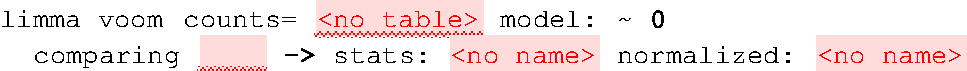
\includegraphics[width=\figWidthWide]{figures/NewLimmaVoom.pdf}
\caption[New Limma Voom Statement.]{\textbf{New Limma Voom Statement.}}
\label{fig:NewLimmaVoom}
\end{figure}


\subsection{Database}
The first Time you will used the \texttt{query Biomart} statement, you will automatically download the available Biomart Databases. They will be stored as an Analysis attributes. To choose your database, go to \textit{select a database} and press control + space.This action will display you all the available database. You will have to choose one from this list. 
\subsection{Dataset}
When a database  is selected, you will download the associated datasets. To choose your datasets you just have to pick up one from the list display when you press control space.
A dataset has two children kinds.
\begin{itemize}
\item attributes which will be the column of your output table
\item filters which allow you to filter your results for some criteria
\end{itemize}
It can append that a dataset is not associated to attributes or filters. If a text \textit{"No available filter or attributes in this dataset"}, that means you need to change your dataset selection or may be the database. 

\subsection{Attributes}
Attributes are the table columns of your futur table. An attribute has three arguments:
\begin{description}
\item [attribute] the attribute name you want to retrieve on the output table
\item [type] the column type of the data. It exist 3 types:
\begin{itemize}
\item string 
\item boolean 
\item numeric
\end{itemize}

\item [Column Group usage] by pressing control space you can choose a group usage define in the Column group Container and add it to your futur table
\end{description}

\subsection{Filters}
Filters are datasets Children. They allow you to filters your results. it exist 4 filters types
\begin{description}
\item[boolean] if this criteria is present or not on your ouput table
\item[text] you have to enter a text in this place for example GO term
\item[list] if this criteria is present, you can filters your results from a set of predifine values
\item[id list] you can restric your results from a set of ids. This ID can come from a Set Of IDs define before the statement, or directly from an annotated with an (ID column) table.  
\end{description}
\subsection{Table}

\section{Example}
%an internet connection 